\documentclass{article}
\usepackage{todonotes}
\usepackage{pbox}
\usepackage{tablefootnote}
\usepackage{setspace}
\title{Dokumentation}
\author{Marc de Bever}
\begin{document}
\maketitle
\tableofcontents

\section{Einleitung}
Dieses Dokument ist ein Teil der Dokumentation des Projektes Imager-Emu\-lator. Dieses Projekt besteht aus drei Teilprojekten. 
Genauer gesagt besteht es aus zwei Bachelor-Thesen und einem Projekt 5 (P5) des Studienganges Elektro- und Informationstechnik der Fachhochschule Nordwestschweiz. 
Das P5 und die erste Thesis laufen parallel, die zweite Thesis wird ein Semester später durchgeführt. Diese Dokumentation ist diejenige von der ersten Thesis, welche parallel mit dem Projekt 5 durchgeführt wird. Das Projekt 5 und die zweite Thesis wird von Fabio Nardo geschrieben und diese Dokumentation ist von mir, Marc de Bever, geschrieben. 

Das Projekt Imager-Emulator wurde von der Firma Varian Medical Systems ausgeschrieben. Das Ziel is es, einen Röntgensensor zu emulieren. Der Sensor wird auch Imager genannt, wenn die ganze zugehörige Elektronik gemeint ist. Daher kommt der Name Imager-Emulator. Der Sensor gibt Bilder über eine nicht standardisierte Schnittstelle an einen Computer weiter. Der Computer, welcher die Bilder des Sensors entgegen nimmt, rechnet diverse Algorithmen, die unteranderem Pixelfehler erkennen und korrigieren. Jedoch kann dem Sensor nicht gesagt werden, \textit{mach mal 'nen Pixelfehler}. Daher braucht es ein Hardware-Emulator, um Bilder mit Pixelfehlern zu generieren und an den Computer zu senden. Mit Hilfe von diesem Emulator können die Algorithmen des Computers in einem realitätsnahen System getestet werden. Der Emulator soll über USB Konfiguriert werden. Somit ergibt sich das Blockdiagramm in Abbildung \ref{fig:bd_sehr_grob}. Ein Computer konfiguriert den Emulator über USB, dieser gibt sich als Imager aus und überträgt die gewünschten Bilder mit den Pixelfehlern auf den XI-Computer. Der XI-Computer ist der Computer, auf dem die Algorithmen laufen. Um die Algorithmen zu testen, bekommt der Computer via Ethernet die berechneten Bilder wiederum  und kann diese mit den erwarteten Bilder verglichen.

\begin{figure}[tb]
    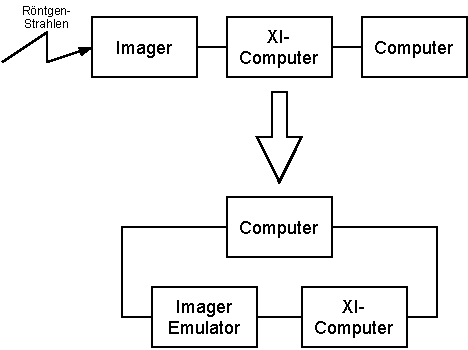
\includegraphics[width=\linewidth]{drawio/bd_sehr_grob}
    \caption{Überblick über das Projekt}
    \label{fig:bd_sehr_grob}
\end{figure}

Da dieses Projekt eine spezielle Konstellation hat, ist die Aufteilung der Teilprojekte wie folgt. Das P5 soll die Hardware entwickeln. Und die erste Thesis, also diese Arbeit, soll die Entwicklungsumgebungen und das FPGA-Modul in Betrieb genehmen, sowie auch die Schnittstellen programmieren. Die zweite Thesis soll schlussendlich die Kommunikation mit dem Computer implementieren, es ermöglichen Pixelfehler in die Bilder einzubauen und das ganze Projekt abzuschliessen.

Dieser Bericht dient zum einen dazu, dass im weiterführenden Projekt verstanden wird, wie die Entwicklungsumgebung und Schnittstellen funktionieren, wo deren Möglichkeiten und Grenzen liegen, und zum anderen dient er, um diese Arbeit als Thesis zu dokumentieren. Der Bericht ist folgendermassen aufgebaut.

Das zweite Kapitel beschreibt wie die Systeme aussehen. Dafür beschreibt es das Projekt mit drei verschiedenen Systemen. Als erstes das, welches von der Varian schon vorhanden ist. Dieses soll durch dieses Projekt emuliert werden. Das zweite System ist eine Zwischenlösung, damit gleichzeitig die Hardware und die Software entwickelt werden kann. Und das letzte System ist das endgültige Gerät, welches den Sensor der Varian emuliert. Diese Kapitel soll einen Top-Down-Blick auf das Projekt geben. Zusätzlich beschreibt es die Wahl des wichtigsten Komponenten, des FPGA-Moduls.

Das dritte Kapitel beschreibt den geschrieben Code. Dieser besteht aus zwei Teilen, der Firmware für den Mikrocontroller und der für den FPGA. Dieses Kapitel erwähnt zum Teil Sachen des zweiten Kapitels nocheinmal. Aber anstatt einen Überblick zu geben, soll dieses Kapitel sich auf die Details konzentrieren.

Das vierte Kapitel beschreibt wie der Imager-Emulator konfiguriert wird und wie zusätzliche Konfigurationen nachträglich hinzugefügt werden können.

Und zu guter Letzt, das fünfte Kapitel beschreibt die Entwicklungsumgebungen (IDEs), mit welchen der Code entwickelt wurde. Dieses Kapitel beschreibt zuerst wie diese aufgebaut sind, was sie können und wie sie zusammenhängen. Als nächstes wird beschrieben, wie man mit den IDEs die Hardware debuggen kann und als letztes die Grenzen der Entwicklungsumgebungen.

\clearpage
\section{System}
Das Projekt kann in drei Systeme unterteilt werden. Das vorhandene System von Varian ist das erste. Das zweite System ist eine Zwischenlösung um mit der Entwicklung der Firmware anzufangen, ohne das die eigene Hardware schon vorhanden ist. Und dass dritte System ist das endgültige System, welches das System von Varian emuliert.

\subsection{System Varian}
\begin{figure}[tb]
    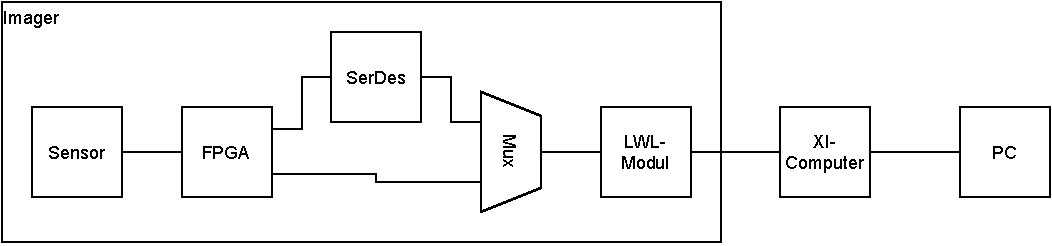
\includegraphics[width=\linewidth]{drawio/bd_varian}
    \caption{Blockdiagramm des Systems von Varian}
    \label{fig:bd_varian}
\end{figure}

Das System der Varian besteht aus dem Imager und dem XI-Computer. Wobei diese beiden Blöcke Teil eines Röntgengerätes für medizinische Zwecke sind. Der Imager ist ein Bildsensor für Röntgenstrahlen und sendet die die gemessenen Bilder über eine LWL-Schnittstelle zum XI-Computer. Der XI-Computer empfängt die Bilder und lässt diverse Algorithmen darüber laufen. Unter anderem auch Algorithmen zur Erkennung von Pixelfehlern. Das mit den Algorithmen bearbeitete Bild wird wiederum über Ethernet an einen externen Computer gesendet.

Um die Bilder vom Sensor auszulesen, zu digitalisieren und zu übertragen, sitzt auf dem Imager ein FPGA. Dieser sendet die Bilder zum XI-Computer ent\-weder über einen vom FPGA internen oder externen Serialisierer/Deserialisierer, kurz SerDes, zu einem LWL-Modul. Der FPGA kommuniziert über einen parallelen Bus mit dem externen SerDes. Die beiden SerDes senden ein LVDS Signal zum LWL-Modul. Das LWL-Modul ist ein standardisiertes Small Form-factor Pluggable (SFP). Um zwischen den beiden SerDes auszuwählen, gehen die Tx-Signale auf einen Multiplexer und die Rx-Signale auf einen Demultiplexer, dieser wird der Einfachheitshalber nur Mux genannt. Das beschriebene System ist im Blockschaltbild in Figure \ref{fig:bd_varian} zu sehen.

Der Vorteil des internen SerDes ist die Geschwindigkeit. Der externe SerDes kann Daten mit einer Übertragungsrate von 1.25Gbps übertragen und der interne mit 6Gbps. Die älteren Versionen des Imagers arbeiten nur mit dem externen SerDes und die neueren mit beiden. Da stellt sich die Frage, wieso überhaupt den externe SerDes brauchen? Beim Einschalten des Imagers ist der FPGA noch nicht konfiguriert und solange der FPGA nicht konfiguriert ist, ist auch der interne SerDes nicht konfiguriert. Somit braucht es den externen SerDes, um den FPGA vom XI-Computer aus zu konfigurieren. Sobald der FPGA konfiguriert ist, schaltet dieser auf den internen SerDes um und kommuniziert mit dem XI-Computer über diesen. Welche SerDes die verschiedenen Versionen des Imagers besitzen ist in Tabelle \ref{tab:sensorVersionen} ersichtlich.

\todo{Unterschied der verschiedenen Versionen erklären}


\begin{table}[tb]
    \caption{Eckdaten der verschiedenen Sensorversionen der Varian}
    \begin{tabular}{|l|l|l|l|l|}
        \hline
        \textbf{Imager} & \textbf{Auflösung} & \textbf{Pattern}$^1$ & \textbf{FPGA} & \textbf{Schnittstelle} \\
        \hline
        DMI$^2$ & 1280x1280 & \pbox[t]{10cm}{b10’1010’1010’1010’1010\\XI: 0xAAA} & \pbox[t]{10cm}{Spartan 3\\XC3S200} & externer SerDes\\
        \hline
        \pbox[t]{10cm}{RTI 1.0$^2$\\(RTI4343L)} & 1280x1280 & \pbox[t]{10cm}{b10’1010’1010’1010’1010\\XI: 0xAAA} & \pbox[t]{10cm}{Spartan 3\\XC3S200} & externer SerDes\\
        \hline
        \pbox[t]{10cm}{RTI 2.0\\(RTI4343iL)} & 3072x3072 &\pbox[t]{10cm}{b10’1010’1001’0101’0101\\XI: 0x955} & \pbox[t]{10cm}{Artix 7\\XC7A100T} & \pbox[t]{10cm}{aktuell:\\externer Serdes\\zukünftig:\\MGT(GTP)} \\
        \hline
        \pbox[t]{10cm}{RTIXL 1.0\\(RTI8643L)} & 6144x3072 & \pbox[t]{10cm}{b10’1010’1001’1001’0101\\XI: 0x995} & \pbox[t]{10cm}{Artix 7\\XC7A200T} & \pbox[t]{10cm}{externer SerDes\\und MGT(GTP)}\\
        \hline
       \end{tabular}
       \begin{tabular}{l}
        {\footnotesize $^1$}\pbox[t]{10cm}{\footnotesize Das XI wertet nur die letzten 12 bit des Pattern aus. Um das DC-Balancing zu erreichen, müssen trotzdem alle 18 bits korrekt gesendet werden.}
        \\
        {\footnotesize$^2$}\pbox[t]{10cm}{\footnotesize DMI und RTI 1.0 besitzen exakt die gleiche Elektronik.}

       \end{tabular}
    \label{tab:sensorVersionen}
    \end{table}

\subsubsection*{Bootvorgang}
\label{sec:varian_boot_sequence}
Das Bitfile um den FPGA zu konfigurieren wird bei jedem Start vom XI-Computer über den externen SerDes auf den FPGA geladen. Dazu müssen sich zuerst die beiden SerDes, also der auf dem Imager und der auf im XI-Computer, synchronisieren. Damit der XI-Computer weiss, welcher FPGA auf dem Imager vorhanden ist, liegt ein Bitmuster mittels Pull-Up und Pull-Down Widerständen an den Tx-Leitungen des SerDes auf dem Imager. Somit ergibt sich folgende Bootsequenz.

Zuerst aktiviert der XI-Computer den Sync-Eingang seines SerDes. Somit kann sich der Rx-Pfad des SerDes auf dem Imager mit dem Tx-Takt des SerDes auf dem XI-Computer synchronisieren. Um dies zu erreichen sendet der SerDes ein Sync-Muster. Der Sync-Eingang des SerDes auf Imagers ist auf einen Rx-Kanal von sich selber angeschlossen. Somit kann der XI-Computer den SerDes auf dem Imager in den Sync-Modus versetzen. Dieser wird, sobald das Rx-Pfade des SerDes auf dem Imager synchronisiert ist, aktiviert. Nun sind beide Pfade der SerDes synchronisiert.

Als nächstes liest der XI-Computer das Versionmuster auf dem Imager aus. Aufgrund von diesem konfiguriert er den FPGA auf dem Imager mit dem entsprechenden Bitfile. Nun ist der FPGA konfiguriert und der Imager kann auf die Befehle vom XI-Computer reagieren. 

\subsubsection*{Kommunikation zwischen Imager und XI-Computer}
\label{sec:varian_com}

Man kann zwischen dem XI-Computer und dem Imager von einer Master-Slave Beziehung reden. Der XI-Computer hat die Möglichkeit dem Imager verschiedene Befehle zu senden, welche der Imager daraufhin ausführt. Es gibt drei verschiedene Gruppen von Befehlen. Es gibt die Write-Befehle, welche dem Imager Einstellungen übermitteln, die der Imager in einem Register speichert. Mit den Read-Befehlen kann der XI-Computer diese Einstellungsregister wieder auslesen. Und als letztes gibt es noch den Trigger-Befehl. Die Write-Befehle beinhalten eine Adresse und einen Wert, die Read-Befehle nur eine Adresse. Mit dem Trigger-Befehl kann der XI-Computer ein Bild anfordern. Ein Trigger-Befehl hat Vorrang vor Write- und Read-Befehlen. Die genaue Auflistung aller Einstellungsregister und deren Aufgabe kann in der Dokumentation des Imagers entnommen werden. \todo{auf Imager Dokumentation referenzieren}

Der FPGA liest immer Zeile für Zeile die Werte des Sensors aus. Solange kein Trigger-Befehl vom XI-Computer gesendet wird, werden die Zeilen verworfen. Sobald ein Trigger-Befehl kommt, wartet der FPGA bis er die letzte Zeile ausgelesen hat und verwirft auch diese noch. Wenn der FPGA nun wieder bei der ersten Zeile angelangt, fängt er an das Bild Pixel für Pixel, Zeile für Zeile zu übertragen. Am Anfang des Bildes vor der ersten Zeile sendet der FPGA ein \textit{Frame-Start} Signal. Und vor jeder Zeile überträgt er ein \textit{Line-Start} Signal. Vor der ersten Zeile muss kein zusätzliches \textit{Line-Start} Signal gesendet werden. Pro Takt wird ein Pixel übertragen. Der FPGA überträgt eine Zeile erst wenn er sie vollständig vom Sensor ausgelesen hat. Dafür überträgt er die Zeile Pixel für Pixel ohne Unterbruch. Ein Pixel ist 16 Bit gross und somit genau gleich gross, wie die parallele Schnittstelle zum SerDes. Um immer eine Zeile vom Sensor auszulesen und eine Zeile zu übertragen speichert ein dual-port RAM die Pixelwerte.

Die Read-Befehle werden nur ausgeführt, wenn keine Bilddaten zu senden sind. Daher werden sie in einem FIFO zwischengespeichert und bei Möglichkeit übertragen. Die Read-Befehle dürfen nur zwischen Zeilen oder Bildern übertragen werden und nicht zwischen einzelnen Pixeln. Da es länger dauert eine Zeile von Sensor zu lesen, als eine Zeile an den XI-Computer zu senden, bleibt immer etwas Zeit um die Read-Befehle vom FIFO abzuarbeiten. Wie vor einem neuen Bild und einer neuen Zeile gibt es das \textit{Command} Signal, dieses wird immer vor der Antwort auf einen Read-Befehls gesendet. Die Antwort eines Read-Befehls bestehen aus den Daten aus dem Einstellungsregister und der entsprechenden Adresse.

\subsubsection*{Wahl des FPGAs}
Das oben beschriebene System der Varian soll emuliert werden. Die Vorgabe ist es 100 Bilder speichern zu können. Mit einer maximalen Bildgrösse von 6144x3072x16 ergibt dies etwa 3.5GB Daten. Als Recheneinheit ist die Vorgabe einen FPGA von Xilinx zu nehmen. Dies ist vom Auftragsgeber, Varian, vorgegeben, da sie mit diesen FPGAs arbeiten und wir somit auch vorhandenen Code für die LWL-Schnittstelle übernehmen können. Die Daten sollen via USB auf das Gerät geladen werden und über die LWL-Schnittstelle weiter zum XI-Computer. Daher braucht das System eine Hardware für das USB und eine für die LWL-Schnittstelle. Für das USB kommt entweder ein externer Chip infrage oder der FPGA muss ein integriertes USB-Modul besitzen. Die LWL-Schnittstell der Varian ist nicht vollständig standardisiert, daher muss diese mit externen Bauteilen aufgebaut werden. Der interne SerDes ist ein Multi-Gigabit-Transiever (MGT). Die FPGAs von Xilinx haben verschiedene MGTs, welche nicht alle die nötigen Geschwindigkeit unterstützen. https://www.xilinx.com/products/technology/high-speed-serial.html\#overview\todo{ref} Das Schema der LWL-Schnittstelle kann von der Varian übernommen werden. Um Übertragungsgeschwindigkeiten bis 6GBps zu unterstützen, muss der Speicher und der FPGA über eine entsprechend schnelle Schnittstelle kommunizieren können. Da das Layouten einer solchen Schnittstellen eine komplexe Angelegenheit ist und bei der Inbetriebnahme zusätzliche Tests benötigt, haben wir uns entschieden ein FPGA-Modul zu verwenden, auf welchem der Speicher schon vorhanden ist. 

Mit diesen Anforderungen haben wir fünf verschiedene Varianten von den Firmen Enclustra und Trenz-Electronic gefunden. Da FPGA-Module mit 4GB RAM sehr teuer sind, haben nicht alle die Kapazität 100 Bilder bei voller Auflösung zu speichern. Die Varianten sind in der Tabelle \ref{tab:modulVarianten} aufgelistet.

\begin{table}[tb]
    \caption{Die verschiedenen Vorschläge für das FPGA-Modul}
    \begin{tabular}{|l|l|l|l|}
        \hline
        & \textbf{Variante 1} & \textbf{Variante 2} & \textbf{Variante 3} \\ \hline

        \textbf{Hersteller} & Enclustra & Trenz-Electronic & Enclustra \\ \hline
        \textbf{Hersteller} & ME-XU5-5EV-2I-D12E & TE0712-02-35-2I & ME-XU5-4EV-1I-D11E-G1 \\ \hline
        \textbf{RAM} & 4GB & 1GB & 2GB \\ \hline
        \textbf{FPGA} & Zynq Ultrascale+ XCZU5EV & Artix-7 & Zynq Ultrascale+ XCZU4EV \\ \hline
        \textbf{USB} & USB 3.0 & - & USB 2.0 \\ \hline
        \textbf{MGT} & 4 MGT 12.5 & 4 GTP & 4 MGT 12.5  \\ \hline
        \textbf{Preis} & 1010 CHF & 225CHF & 680CHF \\ \hline

        \hline
        & \textbf{Variante 4} & \textbf{Variante 5} & \\ \hline
        \textbf{Hersteller} & Trenz-Electronic & Enclustra & \\ \hline
        \textbf{Hersteller} & TE0803-03-4AE11-A & ME-KX1-160-1C-D10 & \\ \hline
        \textbf{RAM} & 2GB & 1GB & \\ \hline
        \textbf{FPGA} & Zynq UltraScale+ XCZU4CG & Kintex-7 & \\ \hline
        \textbf{USB} & USB 3.0 & USB 3.0 & \\ \hline
        \textbf{MGT} & 4 GTH 16.3 & 4 MGT 6.6 & \\ \hline
        \textbf{Preis} & 561CHF & 638CHF & \\ \hline
    \end{tabular}

        
    \label{tab:modulVarianten}
    \end{table}

    Die erste Variante ist die einzige Variante, welches mit 4GB genug Speicherplatz für alle 100 Bilder hat. Dafür ist es auch die teuerste. Das Modul besitzt ein Zynq Ultrascale+ SoC von Xilinx. Der Soc besitzt ein integriertes FPGA-System und ein integriertes ARM Prozessorsystem. Das USB 3.0 ist auch in dem SoC integriert. Somit kann das Prozessorsystem das USB Protokoll abarbeiten, die Bilder auf das RAM laden und das FPGA die Bilder mit der gewünschten Geschwindigkeit zum XI-Computer übertragen.
    
    Variante zwei ist die günstigste, aber hat dafür nur 1GB RAM und kein USB. Als FPGA hat es einen Artix-7. Dies ist ein reiner FPGA und besitzt kein integriertes Prozessorsystem im Gegensatz zu Variante 1. Das USB müsste auf einem vom Modul separaten Chip implementiert werden. 
    
    Varianten drei und vier sind Mittellösungen, sie haben jeweils 2GB RAM und einen Zynq Ultrascale+ SoC. Vom Preis her liegen sie auch in der Mitte. Beide Varianten besitzen ein im SoC integriertes USB. Sie unterscheiden sich im Hersteller des Moduls und in der genauen SoC Version.
    
    Variante fünf ist ist etwa gleich teuer wie die Mittellösungen, jedoch hat sie nur 1GB RAM. Dafür ist sie mit einem einfacheren FPGA und einem externen Chip für das USB ausgestattet. Diese Variante wäre einfacher zu programmieren, da es ein weniger komplexes System ist.

    Die Entscheidung haben wir der Varian überlassen. Die Varian hat sich für die Variante 3 entschieden. Grund für diese Entscheidung ist: "Ein weiteres Entwicklungsboard mit einem Artix-7 bringt uns nichts und ein Modul mit einem Zync Ultrascale+ bringt und auch für später etwas. Ebenfalls gefällt uns, dass bereits DDR4 Memory und USB3.0 vorhanden ist und somit das Preis-Leistungsverhältnis für uns stimmt."

    Jedoch ist uns da noch ein kleiner Fehler unterlaufen. Nämlich hat das Modul der Variante 3 Modul nur USB 2.0 und kein USB 3.0. Das Problem ist, das Enclustra Aufgrund von Kompatibilitäten bei den Mercury XU5 Modulen zwei verschiedene Bestückungsvarianten hat. Die einen führen die GTR-Pins auf die Stecker und die zweite Variante führt mehr IO-Pins anstatt der GTR-Pins auf die Modulstecker. Dies war uns auch so klar. Jedoch braucht das USB 3.0 auch die GTR-Pins, was wir zu diesem Zeitpunkt nicht wussten. Da USB 3.0 auf anderen Leitungen, wie USB 2.0 läuft, aber trotzdem die USB 2.0 Leitung besitzt und unterstützt, können die USB 2.0 Leitungen des SoCs, welche auf anderen Pins heraus geführt werden, trotzdem gebraucht werden. Dies war, obwohl erst nach dem Bestellen gesehen, trotzdem in Ordnung und daher sind wir bei dieser Variante geblieben.
    
\subsubsection*{Enclustra Mercury XU5}
\begin{figure}[tb]
    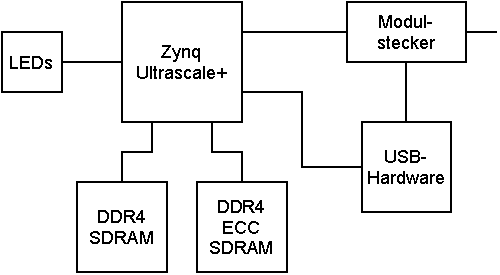
\includegraphics[width=\linewidth]{drawio/bd_xu5}
    \caption{Blockdiagramm SoC Moduls XU5 von Enclustra}
    \label{fig:bd_xu5}
\end{figure}
Das Enclustra Mercury XU5 ist ein SoC Modul, auf welchem ein Xilinx Zynq Ultrascale+ ZU4EV SoC sitzt. 
Der Ultrascale ist ein System on Chip (SoC), welcher ein FPGA-System und ein ARM Prozessorsystem in einem Chip integriert. 
Das Modul hat zwei SDRAMs, wobei einer am ARM System hängt und der andere am FPGA. Beide sind über DDR4 an den SoC angeschlossen. Derjenige, welcher am ARM-System angeschlossen ist, kann mittels einem Error Correcting Code (ECC) zusätzlich noch Fehler erkennen und korrigieren. Dies brauchen wir jedoch nicht. 
Zusätzlich hat es sechs LEDs vier GPIOs und zwei Status-LEDs, welche auf die Pins \textit{PS\_ERROR} und \textit{PS\_STATUS} des SoCs geführt sind. 
Das USB 2.0 vom SoC ist per ULPI mit einem externen Chip auf dem Modul verbunden, welcher wiederum auf die Modulstecker geht. Über zwei Pins des Modulsteckers kann die Bootvariante ausgewählt werden. Somit sind mit vier verschiedenen Boot-Möglichkeiten nicht alle Möglichkeiten des SoCs vorhanden.
Das Blockschaltbild ist in Abbildung \ref{fig:bd_xu5} zu sehen. Das XU5 hat noch weitere Funktionen. 
Diese sind jedoch für dieses Projekt nicht relevant und sind daher weder auf dem Blockdiagramm noch im Text beschrieben. 
Für genauere Informationen kann die Dokumentation des Moduls angeschaut werden. \todo{ref auf Doku von XU5}

\subsubsection*{Xilinx Zynq Ultrascale+}
\begin{figure}[tb]
    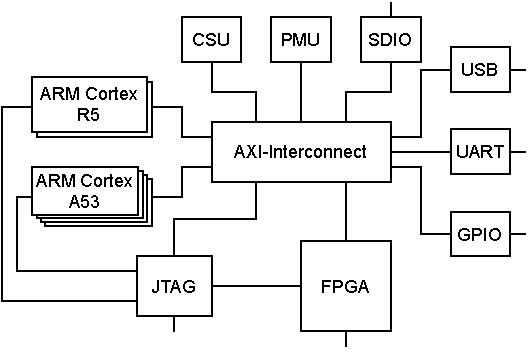
\includegraphics[width=\linewidth]{drawio/bd_soc}
    \caption{Blockdiagramm des Zynq Ultrascale+ SoCs von Xilinx}
    \label{fig:bd_soc}
\end{figure}

Der Ultrascale ist ein SoC mit einem ARM Prozessorsystem und einem FPGA-System integriert in einem Chip. Das ARM-System wird auch Programmable System (PS) genannt und des FPGA-System auch Programmable Logic (PL). Das Blockschaltbild ist in Abbildung \ref{fig:bd_soc} zu sehen. Auch hier sind nur die für das Projekt relevante Blöcke abgebildet. 

Das ARM-System besteht aus zwei ARM Cortex-R5 Kernen, vier Cortex-A53 Kernen und einem Grafikkern. Der Grafikkern ist für das Projekt irrelevant und wird daher komplet verschwiegen. Zusätzlich enthält das ARM-System noch eine Configuration Security Unit (CSU) und eine Platform Management Unit (PMU). Diese beiden Blöcke sind für das Booten zuständig und während dem Betrieb für sicherheitsrelevante Funktionen und das Power Management.

Als Peripherie besitzt der SoC eine Schnittstelle für USB 3.0 und 2.0, UART, SDIO, DDR und JTAG. Zusätzlich können die GPIO Pins als Ein- oder Ausgänge verwendet werden. Die verschiedenen Prozessorkerne. die Peripherien, der Speicher und das FPGA-System sind über AXI-Interconnect-Switches zusammengeschlossen. Das JTAG ist mit drei JTAG-Controllern verbunden. Einer, welcher auf das ganze System Zugriff hat, einer welcher mit dem Coresight des ARM-Systems verbunden ist und einer, welcher das FPGA-System debuggen kann. Das FPGA-System ist ein Xilinx FPGA von der Ultrascale+ Familie. 

Es gibt vier Hauptdokumentationen über das SoC. Das Datenblatt, das Technical Referenz Manual(TRM), die Software Developer Guide und das Packaging and Pinouts Guide.\todo{ref auf Dokus}


\subsection{Entwicklungssystem}
Da das XU5 nur ein Modul ist, welches nicht selbstständig läuft, braucht es ein zusätzliches Board. Im Verlauf dieses Projektes wird dieses Board entwickelt. Damit jedoch direkt von Anfang an mit dem Entwickeln auf dem SoC begonnen werden kann, haben wir zusätzlich noch das Mercury+ PE1-200 Board von Enclustra gekauft. 

\subsubsection*{Mercury+ PE1-200 Baseboard}
\begin{figure}[tb]
    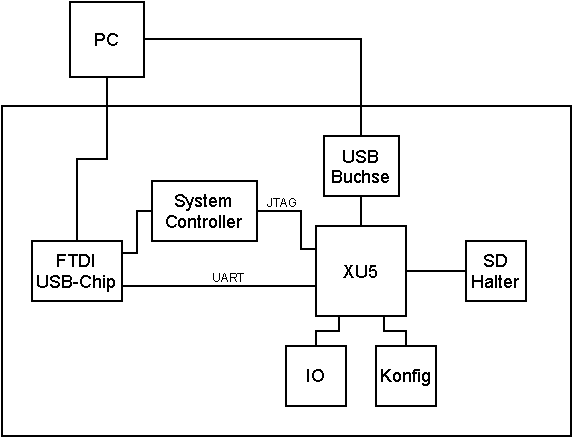
\includegraphics[width=\linewidth]{drawio/bd_pe1}
    \caption{Blockdiagramm des Mercury+ PE1-200 Baseboards von Enclustra}
    \label{fig:bd_pe1}
\end{figure}
Das PE1-Board ist ein Baseboard welches alle zusätzliche nötigen Funktionen für das XU5-Modul zu Verfügung stellt.
Das Blockdiagramm ist in Abbildung \ref{fig:bd_pe1} zu sehen. Auch hier sind wieder nur die für das Projekt relevanten Blöcke zu sehen. 
Das PE1-Board hat zwei USB Ports. Über den einen ist das JTAG und das UART geführt und den zweiten das USB Interface des SoCs. Das Routing der USB Schnittstellen kann über die Schalter auf dem Board eingestellt werden. Das JTAG wird auf einen Chip auf dem Board zu UART umgewandelt, damit mit den Entwicklungsumgebungen direkt ohne zusätzliche Hardware per USB auf die Debug-Schnittstelle zugegriffen werden kann. Ein von Enclustra programmierter Chip konvertiert das JTAG auf UART und ein FTDI-Chip konvertiert die beiden UART-Signale auf USB. Um zu booten wird die SD Karte gebraucht, für welche das PE1-Board eine Halterung besitzt. Zusätzlich hat das Board noch LEDs und Schalter. Die LEDs und Schalter können als IOs des SoCs gebraucht werden. Mit den Schaltern können zusätzlich Einstellungen für den Bootmodus und das Routing der USB-Pfade gesetzt werden. Um von der SD-Karte zu booten, müssen die Schalter \textit{A1} und \textit{B2} abgeschaltet sein. Um das JTAG und UART auf die Mikro-USB-Büchse zu führen, muss Schalter \textit{B2} abgeschaltet sein. Und um das USB-Interface des SoCs auf die USB-B-Buchse zu führen, muss Schalter \textit{B1} abgeschalten sein. 
\todo{ref auf Doku}


\subsection{Endsystem}
\begin{figure}[tb]
    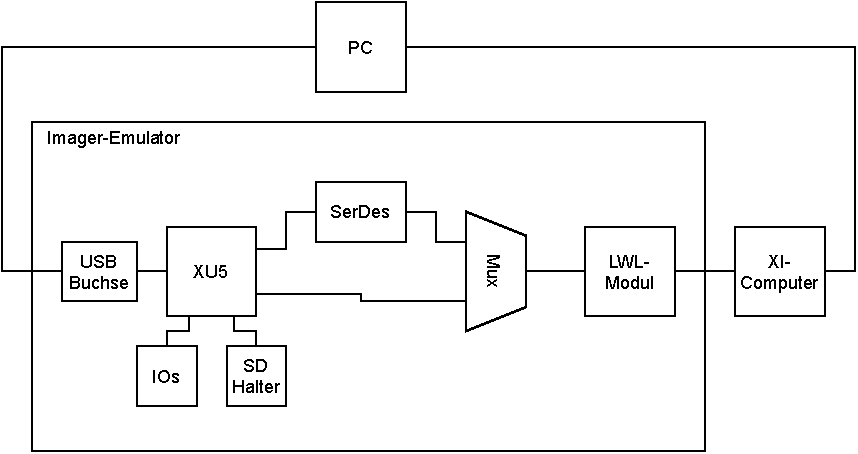
\includegraphics[width=\linewidth]{drawio/bd_top}
    \caption{Blockdiagramm des Imager-Emulators}
    \label{fig:bd_top}
\end{figure}

Das endgültigen System emuliert den Sensor der Varian vollständig. Zuerst durchläuft der Emulator die Bootsequenz des XI-Computers, damit der XI-Computer das Gefühl hat, an einem richtigen Sensor angeschlossen zu sein. Über USB kann man dann den Imager Emulator konfigurieren und die gewünschten Bilder auf den Emulator laden. Der Emulator rechnet anschliessend die Pixelfehler in die Bilder. Auf Befehl vom XI-Computer sendet der Emulator die Bilddaten, oder arbeitet einen Read- oder Write-Befehl ab. Die Pixelfehler werden nach einem vorgegebenen Muster generiert. Die Muster sollen die Zufallsverteilungen der Pixelfehler nachstellen. Da der FPGA die Pixelfehler in die Bilder einbaut, kann das gleiche Bild mit verschiedenen Pixelfehlern verwendet werden, ohne dass zusätzlich Speicherplatz benötigt wird.

In Abbildung \ref{fig:bd_top} ist das Blockschaltbild des endgültigen Systems zu sehen. Das selber entwickelte Board hat einen Stecker für das XU5-Modul. Das Modul kann über den SerDes mit dem XI-Computer kommunizieren. Mit dem Mux kann zwischen dem internen und dem externen SerDes gewechselt werden. Und das SFP Modul wandelt das elektrische Signal in ein optisches um. Die Daten können über den Mikro-USB-Stecker auf den SoC geladen werden. Um zu booten hat es ein SD-Kartenhalter. Zusätzlich hat es noch LEDs und Taster, um, falls nötig, einfache Ein- und Ausgaben zu betätigen. Um zu debuggen hat es einen Stecker für die JTAG-Schnittstelle. Um diese am Computer anzuschliessen braucht es noch eine externe Hardware, welche das JTAG auf USB konvertiert. Die JTAG-Schnittstelle ist nicht auf dem Blockdiagramm, da es nur zu Debug-Zwecken dient und während des Betriebs nicht verwendet wird. 

Dieses Board ist die Arbeit des Projekt 5, welches gleichzeitig mit diesem Projekt durchgeführt. Für eine genauere Erklärung der Hardware und Designentscheidungen wird auf den Bericht jenes Projektes verwiesen. \todo{ref Doku Fabio}

\clearpage
\section{Firmware und FPGA-Code}
%Dieses Kapitel ist der Hauptteil der Arbeit. Es beschreibt den FPGA und Mikrocontroller Code, welcher auf dem SoC läuft und wie dieser getestet wurde. Es ist in die Unterkapitel ARM, FPGA und PC Software aufgeteilt.
%- FPGA Code von Varian mit Blockschaltbild erklären und sagen, welche Module übernommen werden können. Sagen, das der Bootsequenz zuerst noch emuliert wird.
%Blockdiagramm von unserem System zeigen. und in den Unterkapiteln genauer auf die Module eingehen. FPGA code von Varian zuerst nur oberflächlich beschreiben und erst im Unterkapitel FPGA genauer auf die Relevanten Blöcke eingehen.

Der Zynq Ultrascale+ SoC hat ein ARM-Prozessorsystem und ein FPGA-System auf einem Chip. Gebootet wird immer zuerst das ARM-System, welches dann den FPGA konfiguriert. Der Code für das Prozessorsystem nennen wir Firmware und liegt nach dem Bootvorgang auf dem RAM, von wo die Prozessoren auf die Daten und Instruktionen zugreifen. Der FPGA wird mit dem Bitfile geladen, welches den implementierten Code für den FPGA enthält. 

\begin{figure}[tb]
    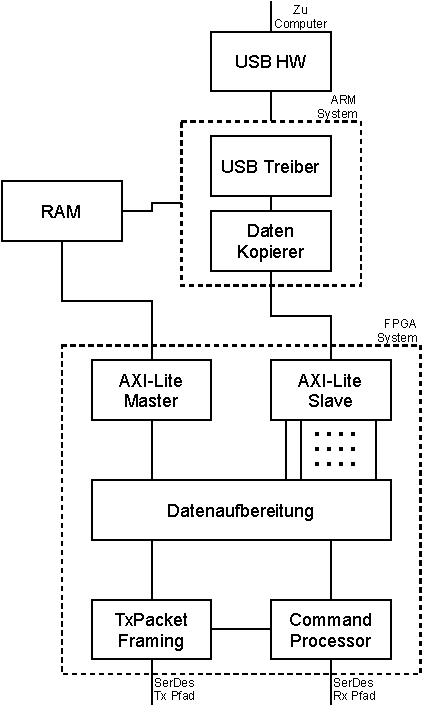
\includegraphics[width=0.6\linewidth]{drawio/bd_firmware}
    \caption{Blockdiagramm der Firmware und FPGA-Codes}
    \label{fig:bd_firmware}
\end{figure}

Abbildung \ref{fig:bd_firmware} enthält das Blockdiagramm vom Aufbau der Firmware und des FPGA-Codes. Vom Prozessorsystem wird nur der ARM Cortex-R5 verwendet. Es gibt zwei Gründe dafür. 

Zum einen ist der Cortex-R weniger komplex als der Cortex-A Kern. Der grösste Unterschied zwischen dem R- und dem A-Kern ist die Memory Management Unit (MMU). Der ARM Cortex-A besitzt eine MMU, welcher den Speicher virtualisiert und den den Zugriff auf jenen Überwacht. Der ARM Cortex-R Kern besitzt nur eine Memory Protection Unit (PMU). Diese virtualisiert den Adressraum nicht, sondern arbeiten mit den physikalischen Adressen. Die PMU überwacht jedoch auch den Zugriff auf den Speicher. Da die Virtualisierung des Adressraums nicht benötigt wird, kann diese Komplexität somit gespart werden. 

Zum anderen liegt der Cortex-R in der Low Power Domain und der Cortex-A in der High Power Domain. Diese beiden Domänen können separat gespeist werden. Somit ist es möglich, die A-Kerne auszuschalten und deren Stromversorgung abzuschalten. Somit reduziert sich der Energieverbrauch des SoCs und somit auch die produzierte Wärme, welche über das Gehäuse dis­si­pie­rt wird.

Der Computer kann über USB die Bilder und die Konfiguration auf das RAM laden. Der \textit{USB Treiber} schreibt diese direkt auf das RAM und benachrichtigt die \textit{Daten Kopier} Funktion, dass neue Konfigurationen vorhanden sind. Auf die Bilder kann der FPGA über eine AXI-Schnittstelle zugreifen mittels dem \textit{AXI-Lite Master} Modul. Die Konfigurationen werden vom ARM direkt auf Register im FPGA geschrieben. Dies passiert auch über eine AXI-Schnittstelle. Die Konfiguration werden sofort in die FPGA-Register geschrieben, damit der FPGA auf alle Konfigurationen parallel zugreifen kann und diese nicht andauernd abfragen muss. Dies übernimmt das \textit{AXI-Lite Slave} Modul.

FPGA-Blöcke \textit{TxPacketFraming} und \textit{CommandProcessor} sind Blöcke, welche wir von dem System der Varian übernehmen können. Jedoch emulieren diese Blöcke die Startup-Sequenz des Sensors nicht. Somit müssen sie noch für unser System angepasst werden. Das \textit{CommandProcessor} Modul empfängt die Befehle des XI-Computers und gibt die Write- und Trigger-Befehle weiter. Die Read-Befehle gibt es direkt an das \textit{TxPacketFraming} Modul weiter. 
%Das \textit{Access Control} Modul speichert die Write-Befehle und gibt Zugriff auf die gespeicherten Konfigurationen und initiiert die Trigger-Befehle. 
Das \textit{Tx Packet Framing} Modul sendet die Daten an den XI-Computer.

Die \textit{Datenaufbereitung} bearbeitet die Bilder mit Pixelfehlern, koordiniert das Senden der Bilder und Arbeitet die Befehle des XI-Computers ab. Dieser Block ist noch nicht Teil von diesem Projekt und wird im nächsten Semester im der weiterführenden Bachelorthesis implementiert.

So soll es auf dem endgültigen System aufgebaut sein. Auf dem PE1-Board also dem Zwischensystem ist es wie in Abbildung \ref{fig:bd_firmware_pe1}. Da der externe SerDes und das SFP-Modul noch nicht vorhanden sind, sind die Blöcke der Varian nicht implementiert. Das Zwischensystem zeigt, dass der PC über USB Daten auf das RAM schreiben kann, dass der ARM-Kern diese Daten über AXI in Register im FPGA schreiben kann, und dass der FPGA über AXI auf das RAM zugegriffen kann. Um dies zu zeigen, ist das Register, auf welches der ARM-Kern schreibt, mit einem LED verbunden und das \textit{AXI-Lite Master} Modul mit zwei LEDs, welche anzeigen, ob der Schreib- und Lesezyklus fertig ist und ob er erfolgreich war. Zudem gibt der ARM-Kern über UART den Wert des RAM-Registers und des FPGA-Registers aus. Über einen DIP-Switch kann man den Wert einstellen, welcher das FPGA in das RAM schreiben soll. 

\begin{figure}[tb]
    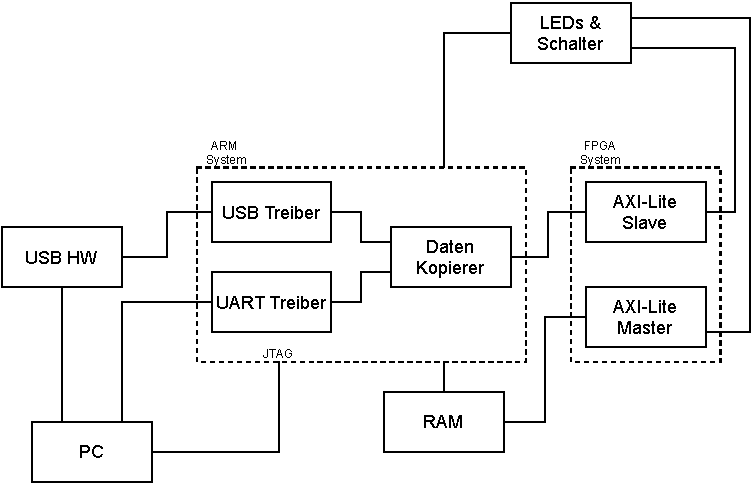
\includegraphics[width=\linewidth]{drawio/bd_firmware_pe1}
    \caption{Blockdiagramm der Firmware und FPGA-Codes auf dem Entwicklungssystem}
    \label{fig:bd_firmware_pe1}
\end{figure}

\subsection{Bootvorgang}



\subsection{ARM Firmware}
Die Firmware für den ARM Cortex R5 besteht aus vier Teilen. Dem \textit{USB-Treiber}, der \textit{Daten Kopierer} Funktion, dem \textit{IO-Treiber} und der \textit{Main} Funktion. Den \textit{USB-Treiber} haben wir von Xilinx übernommen und ein wenig angepasst. Der \textit{Daten Kopierer} hat eine Struktur, welche die Konfigurationen auf die Register in FPGA schreibt, sobald der \textit{USB-Treiber} meldet, dass die Konfigurationen geändert wurden. Über den \textit{IO-Treiber} kann man die LEDs, Taster und Schalter ein- und auslesen, ohne sich Gedanken über die physikalische Anordnung der IOs zu machen. Die \textit{Main} Funktion verbindet die Blöcke und gibt für Testzwecke Informationen über UART oder die LEDs weiter.

\subsubsection*{USB-Treiber}
Der \textit{USB-Treiber} ist das grösste Modul der ARM-Firmware. Daher wird diese ein wenig genauer beschrieben. Leider hat sich Xilinx nicht viel Aufwand für das Konzept, die Lesbarkeit und die Dokumentation des USB-Treibers gemacht.

Der \textit{USB-Treiber} verwendet zum einen den USB-Treiber, welcher im Board Support Package (BSP) im Platform Projekt von Vitis vorhanden ist. Und zum anderen das Beispiel Projekt, welches Xilinx mit dem Treiber mitliefert. Der USB-Treiber des BSPs hat Funktionen und Datenstrukuren, um die Grundlegenden Funktionen des USB-Moduls zu steuern. Das Beispielprojekt implementiert den Softwareteil des USB-Standards und der Massstorage USB-Klasse. Das Beispielprojekt unterstützt den reduzierten SCSI Befehlssatz, um die Massstorage Klasse zu implementieren.

Das Beispielprojekt greift auf die Funktionen des USB-Treibers des BSPs über eine Wrapper-Library zu. Diese Bibliothek ändert die API des USB-Treibers des BSPs. Jedoch greift das Beispielprojekt trotzdem noch direkt auf den USB-Treiber des BSPs zu. 
\subsubsection*{ARM Konfiguration}
\todo{MPU und andere Einstellungen beschreiben}

\subsection{AXI Protokoll}

\subsection{AXI FPGA-Module}
\label{sec:axi}
Die AXI FPGA-Module sind Vorlagen von Xilinx. Der AXI-Lite Slave nimmt Daten über das AXI Protokoll entgegen, speichert diese in Registern im FPGA und gibt die Daten wieder aus, wenn ein entsprechender AXI-Befehl ankommt. Der AXI-Lite Master schreibt sequenziell über AXI auf eine Reihe von Registern und liesst diese anschliessend wieder aus und vergleicht sie mit den geschriebenen Werten. Beide Module implementiereren die AXI-Protokolle, indem sie für jeden Ausgang einen VHDL-Prozess definieren, welcher den Wert des Ausgangs anhand von den Eingängen bestimmt. Wenn die Eingänge zu wenig Information geben um die Zustände des Ausgangs komplet zu beschreiben, führen sie noch Zwischensignale ein.


\subsection{Varian FPGA-Module}
Die beiden Module \textit{TxPacketFraming} und \textit{CommandProcessor} sind von der Firma Varian geschrieben. Für dieses Projekt können wir sie grössten Teils übernehmen. Abbildung \ref{fig:bd_fpga_varian} zeigt das Blockschaltbild der beiden Module und wie sie zusammengehängt sind.

\begin{figure}[tb]
    \missingfigure{Blockschaltbild}
    \caption{Blockdiagramm der beiden Module \textit{TxPacketFraming} und \textit{TxPacketFraming}}
    \label{fig:bd_fpga_varian}
\end{figure}

\subsubsection*{TxPacketFraming}
Das Modul \textit{TxPacketFraming} ist zuständig für die Übertragung der Daten an den XI-Computer über den externen SerDes. Da der externe SerDes eine DC-freie codierung besitzt, muss dies im FPGA geschehen. Dafür werden die Daten zuerst vom \textit{Encoder} Modul kodiert, bevor sie an den SerDes gesendet werden. Das \textit{Encoder} Modul hat vier Eingänge und einen Ausgang.
Der \textbf{Clk}-Eingang ist der Takt des Moduls.
Der \textbf{Code}-Eingang zeigt, ob es sich um ein Signal oder um Bilddaten handelt.
Der \textbf{En}-Eingang aktiviert das Modul.
Im \textbf{DataIn}-Eingang werden die Daten und Signale eingegeben.
Der \textbf{DataOut} Ausgang gibt die codierten Daten und Signale aus.

Der Imager sendet entweder Bilddaten oder Antworten von Befehlen des XI-Computers. Vor jedem neuen Bild sendet der Imager ein \textit{Frame Start} Signal, vor jeder neuen Zeile eines Bildes eine \textit{Line Start} Signal und vor jeder Antwort eines Befehls ein \textit{Command} Signal. Wie in Kapitel \ref{sec:varian_com} unter \textit{Kommunikation zwischen Imager und XI-Computer} erläutert.

Der Tx-Pfad des SerDes hat 18 parallele Bits. 16 werden gebraucht, um die Daten und Signale zu übertragen, eines um zu signalisieren, ob es sich um ein Signal oder um Daten handelt und das letzte, um das DC-Balancing zu implementieren.

Die Antworten auf einen Read-Befehl werden vom \textit{CommandProcessor} mit den Eingängen \textbf{TxCmdWrite} und \textbf{TxCmdData} in ein Fifo geschrieben und bei Gelegenheit, zwischen den Bildzeilen, Übertragen.
Um eine Bildzeile zu übertragen muss der Eingang \textbf{ImgDataReady} gesetzt werden und den \textbf{FrameLineStart}-Eingang entsprechend gesetzt werden. Für ein neues Bild muss \textit{0b10} und für eine neue Zeile \textit{0b01} angelegt werden. Wenn das \textit{TxPacketFraming} Modul bereit ist die Zeile zu übertragen bestätigt es dies mit dem Setzen des Ausgangs \textbf{ImgDataRdEn}. Im nächsten Takt überträgt das Modul das Signal und danach überträgt es pro Takt einen Pixel. Dafür müssen die Pixeldaten am Eingang {ImgData} angelegt werden und mit jedem Takt entsprechend dem nächsten Pixel erneuert werden. Sobald alle Pixel der Zeile übertragen sind muss der \textbf{ImgDataReady}-Eingang gelöscht werden. Am \textbf{Clk}-Eingang muss der Takt angelegt werden und der Ausgang \textbf{TxDataOut} geht auf die Pins, welche mit dem Externen SerDes verbunden sind.

Dieses Verhalten ist mittels einer Finite State Machine (FSM) gelöst. Die FSM ist in Abbildung \ref{fig:fsm_tx_packet_framing} zu sehen.

\begin{figure}[tb]
    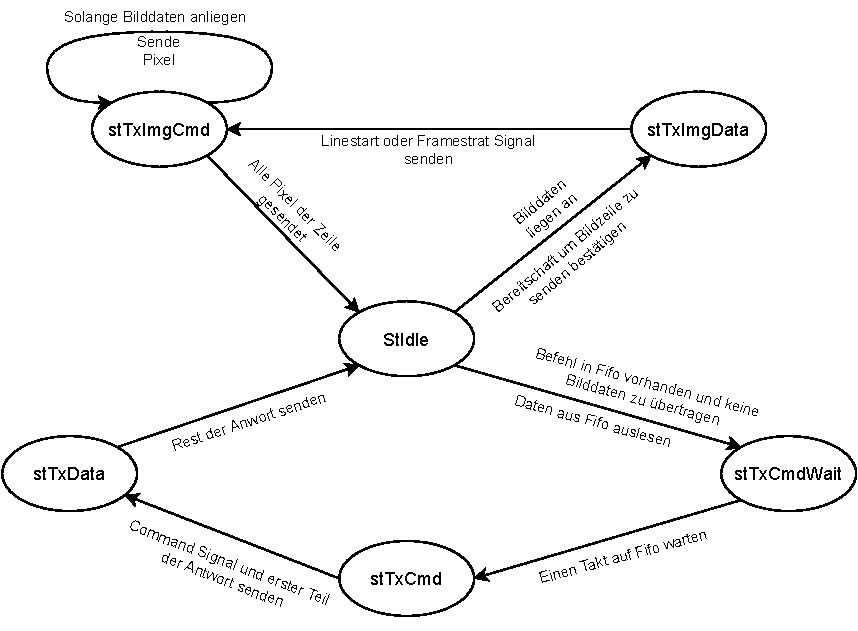
\includegraphics[width=\linewidth]{drawio/fsm_tx_packet_framing}
    \caption{State Machine des Moduls \textit{TxPacketFraming}}
    \label{fig:fsm_tx_packet_framing}
\end{figure}

\subsubsection*{CommandProcessor}
Das Modul \textit{CommandProcessor} beinhaltet das Modul \textit{RxPacketframing}.Dieses beinhaltet wiederum zwei Fifos. Eines direkt am Rx-Eingang vom SerDes, welches zwischen dem FPGA-Takt und dem SerDes-Takt wechselt. Und eines um die Daten für den \textit{CommandProcessor} bereit zu stellen. Das erste Fifo ist nur aktiv, wenn das SFP und der SerDes parat sind. Dafür sind die Eingänge \textbf{nSerdesLock} und \textbf{OptoSD}. Zudem wird eine UND-Verküpfung der beiden Signale am Ausgang \textbf{OptlinkReady} ausgegeben. Das Modul \textit{RxPacketframing} unterscheidet zwischen den drei verschiedenen Befehlen des XI-Computers. Ein Trigger-Befehl gibt es direkt an den Ausgang \textbf{Triggerlines}. Und die Read- und Write-Befehle schreibt es in das zweite Fifo. Wenn das erste Bit eine "0" ist, handelt es sich um einen Read-Befehl und ansonsten um einen Write-Befehl. Die nächsten sechs Bits im Fifo geben die Adresse de Read- oder Write-Zugriffs an. Und die zwei Byte sind nur für den Write-Befehl relevant und entahlten die zu schreibenden Daten. Dieses Verhalten ist in der FSM in Abbildung \ref{fig:fsm_tx_packet_framing} zu sehen.

\begin{figure}[tb]
    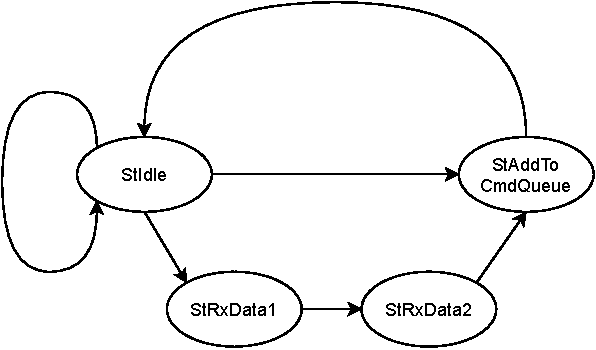
\includegraphics[width=\linewidth]{drawio/fsm_rx_packet_framing}
    \caption{State Machine des Moduls \textit{RxPacketFraming}}
    \label{fig:fsm_rx_packet_framing}
\end{figure}

Der \textit{CommandProcessor} nimmt die Daten aus dem Fifo und arbeitet diese ab. Wenn es sich um einen Write-Befehl handelt, sendet er die Daten zu den Einstellungsregistern. WEnn es sich um einen Read-Befehl handelt liest er die Daten von den Einstellungsregistern und gibt die Daten über die Ausgänge \textbf{TxCmdWrite} und \textbf{TxCmdData} and das Fifo des Moduls \textit{TxPacketFraming} weiter.

Die Schnittstelle zu den Einstellungsregistern besteht aus den den Ausgängen \textbf{WrEn}, \textbf{AddrBus}, \textbf{DataWrBus} und aus den Eingängen \textbf{DataRdBus}, \textbf{Ready}.
Wenn der Ausgang \textbf{WrEn} gesetzt ist, handelt es sich um einen Write-Zugriff und ansosten um einen Read-Zugriff. Sobald der Eingang \textbf{Ready} gesetzt wird, heisst es, dass der Zugriff erfolgreich war. Der \textbf{Ready} Eingang wird erst ein Takt nach dem anlegen der Adresse und der Daten geprüft. Die Adresse wird am Ausgang \textbf{AddrBus} angelegt, die zu schreibenden Daten an dem \textbf{DataWrBus} und die zu lesenden Daten werden vom Eingang \textbf{DataRdBus} gelesen. Dieses Verhalten ist mit der FSM in Abbildung \ref{fig:fsm_command_processor} implementiert.

\begin{figure}[tb]
    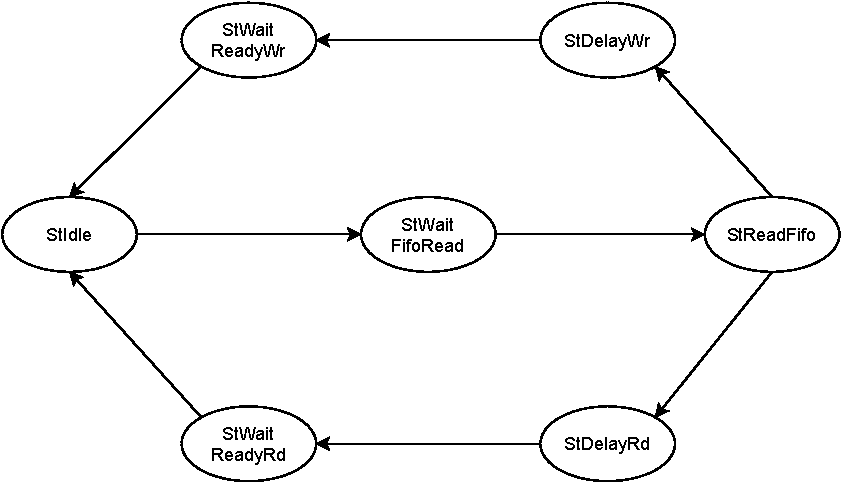
\includegraphics[width=\linewidth]{drawio/fsm_command_processor}
    \caption{State Machine des Moduls \textit{CommandProcessor}}
    \label{fig:fsm_command_processor}
\end{figure}

\subsection{Vivado Projekt}
Das Vivado Projekt kann mit dem Skript erstellt werden. Das Skript kreiert ein neues Projekt, erstellt ein Blockdiagramm im IP Integrator, fügt alle Blöcke in das Blockdiagramm, konfiguriert das Prozessorsystem im Blockdiagramm, erstellt die Top-Datei und es erstellt die Constraint-Datei.

Die Top-Datei instantiiert das Blockdiagramm vom IP Integrator und definiert die Namen der Ausgänge, welche an die Pins gehen. Die Constraint-Datei verbindet die Ausgänge der Top-Datei mit den Pins und konfiguriert die Pins entsprechend. 

\subsection{Vitis Projekt}
Das Vitis Projekt kann auch mit einem Skript erstellt werden. Das Skript erstellt mit der exportierten XSA-Datei ein Plattform Projekt und kompiliert dieses. Wenn nur ein aktualisierter Bootloader gebraucht wird, reicht es, das Skript bis hier auszuführen. Danach erstellt das Skript die Applikation und kopiert die Sourcefiles hinein. Am Schluss kompliert es die Applikation und erstellt ein Bootimage.

\section{Imager-Emulator Konfiguration}
Die Konfigurationen können über USB auf den Imager-Emulator geladen werden. Die Daten sind im RAM in einer C-Struktur gespeichert. Im Moment hat die Struktur vier Einträge. Der \textbf{Enable}-Eintrag kann den Emulator stoppen. Die Idee ist, dass immer wenn der PC neue Konfigurationen und Bilder auf den Emulator lädt, dieses Bit zuerst gelöscht wird und somit der Emulator stoppt. Dies soll mögliche Fehler verhindern, welche wegen unvollständigen Konfigurationen und Bilder entstehen können. Sobald der Emulator vollständig konfiguriert ist, setzt der PC dieses Bit wieder. Der \textbf{n}-Eintrag gibt an wieviele Bilder auf dem Emulator gespeichert sind. Der \textbf{StartAddr}-Eintrag sagt, wo das erste Bild im RAM anfängt. Und der \textbf{Bildgrösse}-Eintrag sagt mit drei Bits welche Bildgrösse die Bilder haben. Somit kann das FPGA ausrechnen, wann das nächste Bild anfängt. Diese Konfigurationen sind an erster Stelle im ersten Sektor des USB-Massenspeichers. Das USB-Massenspeicher Protokoll definiert, dass immer ein Sektor aufs mal gschrieben wird. Ein Sektor ist 512 Byte gross. Sobald im ersten Sektor etwas geschrieben wird, aktuallisiert das ARM-System die Register auf dem FPGA.

Um neue Konfigurationen hinzzufügen muss lediglich die C-Struktur um dîe Konfiguration erweitert werden. Die Funktion, welche die Konfigurationen auf die FPGA-Register schreibt, kopiert dann diese Struktur. Zudem muss diese Struktur in der PC-Applikation nachgebildet sein, damit die Konfigurationen auch in der richtigen Reihenfolge auf den Massenspeicher geschrieben werden.

\section{Entwicklungsumgebung}
Es gibt zwei Entwicklungsumgebungen (IDE) von Xilinx, um den Zynq Ultrascale+ SoC zu programmieren und zu konfigurieren. Die eine ist Vivado. Vivado ist die IDE um Code für den FPGA zu entwickeln. Mit Vivado kann man IPs im Projekt einfügen, FPGA Code simulieren, syntetisieren, implementieren, den FPGA Konfigurieren und direkt auf dem FPGA debuggen.

Die zweite IDE ist Vitis. Mit Vitis kann man Code für das ARM-System schreiben, Bootdateien erstellen, das ARM-System programmieren, den FPGA konfigurieren und den ARM debuggen. Vitis basiert auf der Eclipse IDE mit den GNU GCC Tools.

In diesem Projekt wurden die Versionen 2019.2 von Vivado und Vitis verwendet. Es ist die erste Version von Vitis. Vorher wurde die Xilinx SDK verwendet um Code für den ARM zu schreiben. Ab Vivado 2019.2 ist es jedoch nicht mehr möglich Projekte für die SDK zu exportieren, da die SDK und Vitis unterschiedliche Files brauchen um die Hardware, welche mit Vivado generiert wird, zu importieren. Für beide Tools können mit TCL Skripte geschrieben werden.

Mit den beiden Entwicklungsumgebungen kommt noch das Programm DocNav. Diesem Programm beinhaltet alle Dokumentationen von Xilinx.
\subsection{Vivado}
Vivado ist die IDE für die Entwicklung von FPGAs, sie versteht VHDL und Verilog. Vivado kann entweder im Projektmodus oder nicht im Projektmodus verwendet werden. In diesem Projekt verwenden wir Vivado nur im Projektmodus. Alle Befehle können enteder im GUI oder in der TCL Konsole eingegeben werden. Somit ist Vivado vollständig skriptbar. Ein Vivadoprojekt besitzt ein Top-Modul, welches alle anderen Module und Blockdiagramme hinzufügt.

Vivado besteht aus verschiedenen Teilprogrammen. Diese sind der IP-Integrator, der Simulator, der Syntetisierer, der Implementierer und der Hardwaremanager.

Die Dokumentation von Vivado ist auf verschiedene Dokumente aufgeteilt. Zum Starten ist die "Vivado Design Suite User Guide: Using the Vivado IDE" gut geeignet. Diese Dokumentation referenziert in Kapitel zwei auf die weiteren Dokumentationen der einzelnen Unterprogramme von Vivado. \todo{ref auf Doku}

Der IP-Integrator ist das Tool um die Intellectual Properties (IP) zu instanzieren. Dafür erstellt der IP-Integrator ein Blockdiagramm, welches ein VHDL-Modul einbinden kann. Das Blockdiagramm kann auch selber erstellt IPs und VHDL-Module beinhalten, wobei hier die Grenze zwischen IP und VHDL-Modul schwimmend sind. Der Wizard "Create and Package new IP" kann die eigene Module in IPs umwandeln, aber muss nicht um es im Blockdiagramm des IP-Integrators einzufügen. Zudem hat der Wizard Vorlagen für AXI-Schnittstellen. Diese sind in Kapitel \ref{sec:axi} genauer beschrieben. Der Wizard kann man in der Menuleiste unter Tools starten. Das IP \textit{zynq\_ultra\_ps} instanziert das Prozessorsystem des Ultrascales. Somit kann man dieses konfigurieren und die anderen IPs an die Schnitstellen zum PS anhängen. Die Konfigurationen exportiert Vivado mit der XSA-Datei, mit welchem Vitis dann die Plattform generiert. \todo{ref auf Doku}

Der Simulator simuliert die VHDL Module(Mindblowing). Für die Simulation können mehrere Sets definiert werden, welche man von einander getrennt aufrufen kann. Die Testbenches können direct auf die Module im Projekt zugreifen. \todo{ref auf Doku} 

Der Syntetisierer und Implementierer generieren das Bitfile für das Konfigurieren des FPGAs. Dabei ist der Syntetisierer der Hardware unabhängige Teil und der Implementierer der Hardware abhängige. Die XDC-Constraint-Dateien konfigurieren diese beiden Tools. In den Constraint-Dateien müssen auch die Zuweisung der Ein- und Ausgänge des Top-Moduls zu den Pins und deren Einstellungen statfinden. \todo{ref auf Doku Imp, Synt, Const}

Der Hardware Manager kann den Bitstream direkt auf den FPGA laden und debuggen. Dfür braucht es jedoch noch einen oder mehrere Integrated Logic Analyser (ILA) IPs, welche im Blockdiagramm eingefügt werden können. Mit diesen kann man auf ein Trigger die gewünschten Signale für eine gewisse Zeit anschauen. \todo{ref auf Doku HM, ILA}

\subsection{Vitis}

\begin{figure}[tb]
    \missingfigure{Zusammenhänge der verschiedenen Vitis-Projekten}
    \caption{Zusammenhänge der verschiedenen Vitis-Projekten}
    \label{fig:vitis}
\end{figure}

Vitis ist die IDE von Xilinx, um das Prozessorsystem zu programmieren. Vitis bassiert auf der Eclipse IDE. 
Von Vivado kann man die Hardware exportieren und in Vitis importieren. Mit der importierten Hardware wird ein Plattform-Projekt generiert. Diese Plattform beeinhaltet Domainen und die Domainen wiederum Board Support Packages, welche die Bibliotheken und Peripherietreiber beinhalten. Jede Domaine ist für einen bestimmten Prozessorkern. Es können verschiedene Domainen für die selben Kerne existieren, wobei diese nicht die gleichen Einstellungen der Bibliotheken haben müssen. Zudem gibt es noch zwei spezielle Domainen. Eine Domaine für den First Stage Boot Loader (FSBL) und eine für die Firmware der Platform Management Unit (PMU). Auf Grund von den Plattformen kann man Projekte erstellen. Hier gibt es auch zwei verschiedene Arten. Die Applikations-Projekte und die System-Projekte. Jedes System-Projekt kann mehrere Applikations-Projekte enthalten. Jedoch pro ProcessorKern nur eines. Jedes System-Projekt ist an ein Platform-Projekt gebunden und jedes Applikations-Projekt an eine Domaine und befindet sich in einem System-Projekt.

Kompiliert wird der Code mit den GCC Compilern. Diese werden mit Vitis mitinstalliert und können von Vitis aus gestartet werden. Der Compiler generiert ELF-Dateien, welche auf den SoC geladen werden können. Die Erfahreung hat gezeigt, dass Vitis stabiler läuft, wenn zuerst das Platform-Projekt compiliert wird und erst danach die System- und Applikations-Projekte. Falls jedoch die Plattform nicht verändert wurde und sie nicht veraltet ist, muss sie nicht notwendig compiliert werden.

Das Bootgen Tool generiert aus den ELF-Dateien und Bitfiles ein bootbares Image. Mit diesen kann man den SoC booten. Dafür muss es entweder auf die SD-Karte geschrieben werden, oder über JTAG auf den SOC geladen werden. Zusätzlich kann mit dem Tool Program Flash das Bootimage auf das externe Flash des SoCs laden. Dafür wird das File über JTAG and das Flash übertragen.

Mit dem Xilinx Software Command-Line Tool (XSCT) können auch Skripte für Vitis geschrieben werden. Die XSCT kann entweder in Vitis geöffnet werden, oder direkt in einem Terminal. Das XSCT basiert wie Vivadoskripts auf TCL.

Die Dokumentation von Vitis ist unter \todo{ref auf doku} zu finden.

\subsection{Schnittstelle zwischen Vivado und Vitis}



\subsection{No Gos}
XSA Datei in Vitis Aktualisieren\\
Projekte kopieren, da zum Teil absolute Pfade verwendet werden\\
Bitstream nicht mit Hardware exportieren\\
Nicht die richtige Reihenfolge im Bootgen Tool\\
richtige Reihenfolge: -PMU\\
- FSBL\\
- Bitfile\\
- restliche ELF-Files


\section{Reflexion}



\section{Erläuterungen}
Dieses Kapitel listet alle Abkürzungen mit den Bedeutungen und einer kurzen Erklärung auf. Zudem erklärt es, wie die verschiedenen Fachwörter zu verstehen sind.

ARM Core,
Core,
FPGA,
Sensor,
XI-Computer,
SoC,
Imager,

Imager-Emulator

P5
LWL
FPGA
Imager
XI-Computer
SerDes
LVDS
Rx
Tx
FIFO




\end{document}